\begin{frame}[t]{DATEN}
  \begin{columns}
    \begin{column}{0.3\textwidth}
      \centering
      \begin{tikzpicture}[scale=0.9]
        \node[anchor=south west,inner sep=0] at (0,0)
          {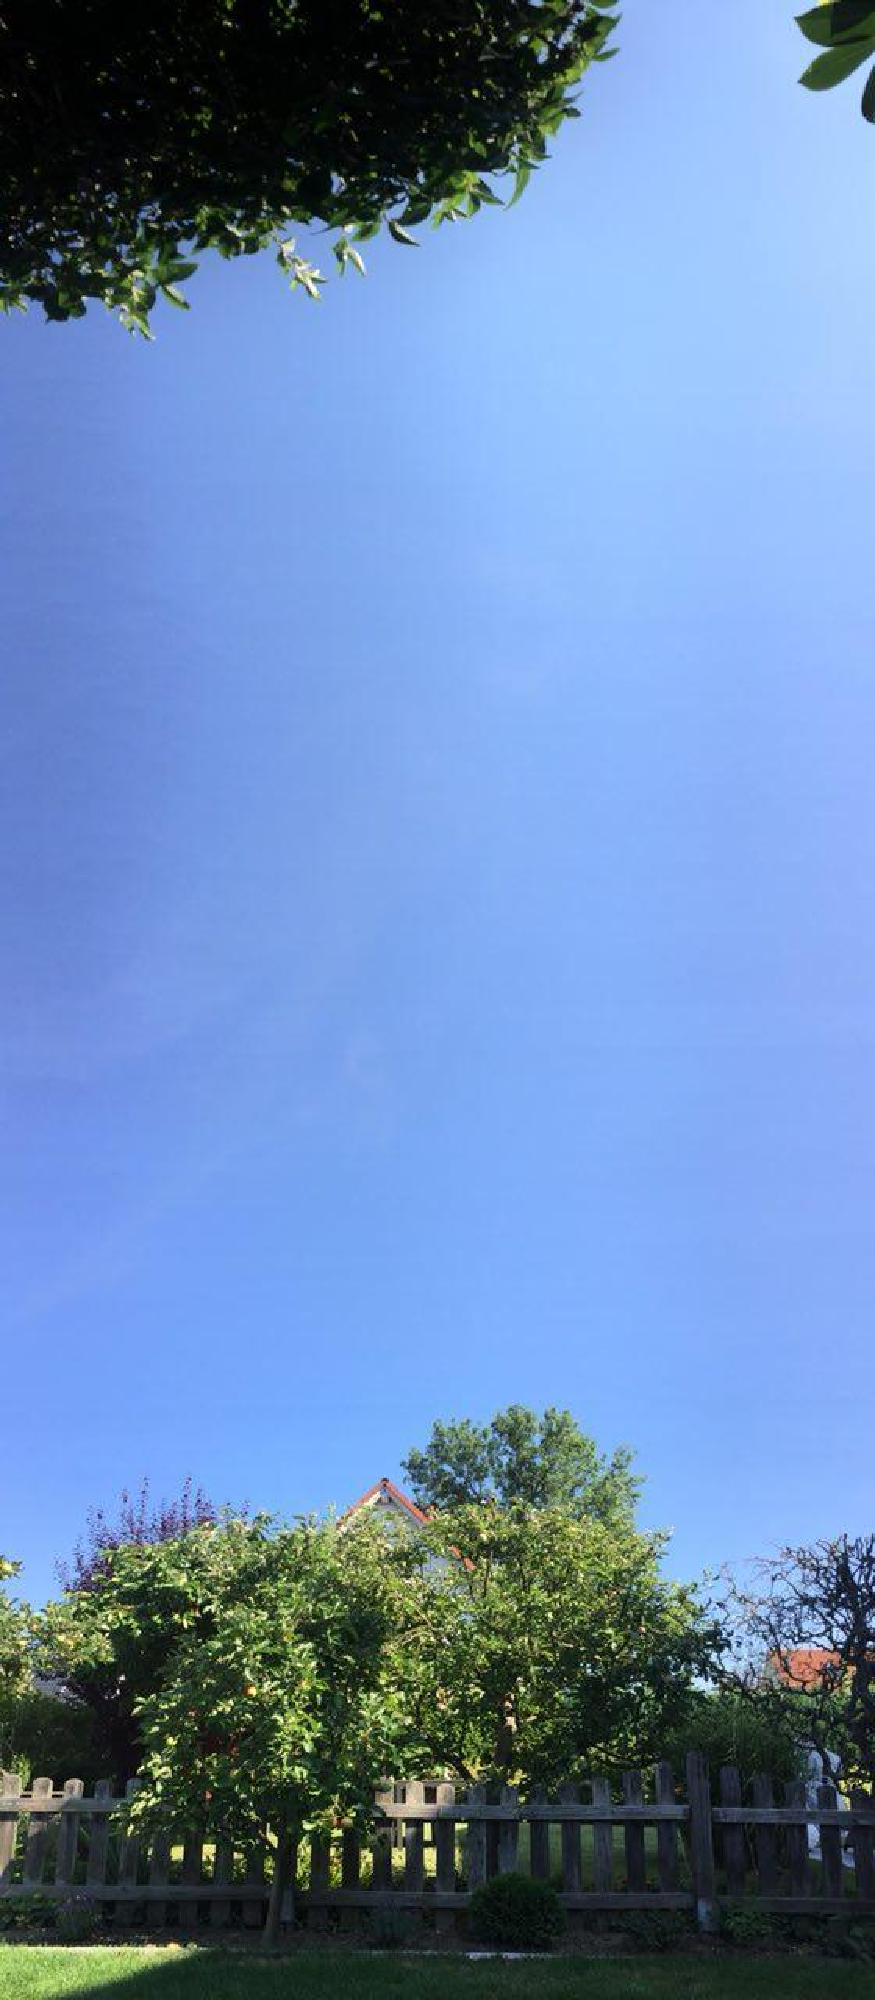
\includegraphics[width=0.9\textwidth]{content/station_winkel.pdf}};
        \draw[red, line width=0.04cm, rounded corners] (0,2) rectangle (\textwidth, 4)
          node[below left, black]{$\Omega_1$};
        \draw[red, line width=0.04cm, rounded corners] (0,4) rectangle (\textwidth, 6)
          node[below left, black]{$\Omega_2$};
        \draw[|->, thick] (-0.3,0) node[left]{\SI{0}{\degree}} to ++(0, 8)
          node[below left]{\SI{180}{\degree}} node[right]{$\omega$};
      \end{tikzpicture}
    \end{column}
    \begin{column}{0.7\textwidth}
      \begin{itemize}
        \item 4000 Fotos
          \begin{itemize}
            \item Nachtfotos entfernen
            \item Idee: Zeit
            \item[$\Rightarrow$] Aber: Helligkeit
          \end{itemize}
        \item Unterschiede $\Omega_i$
          \begin{itemize}
            \item verschiedener Blick auf Wolken
            \item Anzahl an Wolken
          \end{itemize}
      \end{itemize}
    \end{column}
  \end{columns}
\end{frame}
